
\documentclass[16pt,twocolumn,letterpaper,titlepage]{article}
\usepackage{apacite}
\usepackage{tablefootnote}
\usepackage{titling}
\usepackage{graphicx}
\usepackage[T1]{fontenc}
\usepackage{babel}

\usepackage{titlesec}% http://ctan.org/pkg/titlesec
\titleformat{\section}%
  [hang]% <shape>
  {\normalfont\bfseries\Large}% <format>
  {}% <label>
  {0pt}% <sep>
  {}% <before code>
\renewcommand{\thesection}{}% Remove section references...
\renewcommand{\thesubsection}{\arabic{subsection}}%

\setlength{\droptitle}{-12em}  
\setlength\bibitemsep{\baselineskip}
\title{Experimenting With Scalable Forecasting Models}

\author{
    Matthew Coghlin\\
  	\and
  	Pelumi Dacosta\\
    \and
    Joseph Despres\\
    \and
    Aneesh Ghai\\
    \and
    Joseph Sigler\\
}

\begin{document}


\maketitle


\onecolumn
\tableofcontents
\thispagestyle{empty}
\newpage
\twocolumn
\bibliographystyle{apacite}

\setcounter{page}{1}

\section{Introduction}

Organizations planning for the future need to reliably estimate the future value of many variables. Estimating retail demand to planning inventory, customer arrivals for staffing decisions, and estimating input costs for budget allocations, all depend on forecasts. Forecasting is the practice of using current data available to estimate the value of a future variable at a time that has not yet happened. Decision-makers in government, business, and non-profit organizations require accurate and reliable forecasts. However, there are tremendous costs associated with forecasts that are either too high or too low. Such as a store running out of inventory, unable to checkout enough shoppers, or left with rotting produce. Therefore, it is essential to minimize forecasting error. However, there is a growing number of items to forecast, and manually forecasting each series will not scale. Therefore, this project implements methods for generating high-quality, reliable forecasts for many series. 


As data becomes cheaper to store and more convenient to collect, organizations have the opportunity to improve forecasts. To obtain a reliable forecast, a time-series expert was generally required to carefully tune model parameters and make judgments on which models to implement \cite{taylor2018forecasting}. Although this approach is rigorous, it does not scale. Any standard grocery store has enough items to overwhelm anyone manually tuning and selecting forecasting models. Analysts could need to generate high-quality forecasts for thousands and even hundreds of thousands of series at a time. The goal of this project is to implement forecasting algorithms that generate high-quality forecasts with minimal involvement, validate them with a training and testing partition, and generate ensemble predictions made up of the various forecasts.


We begin with a discussion of the data and metrics used to evaluate forecasts. Then we specify the requirements for the models to be used for this task. Then briefly explain the intuition of each model and give reasons for selecting them. Then we discuss model performance on testing data. After that, we discuss our Kaggle challenge and the various approaches we took when making submissions. We conclude with some remarks on the process and how these applications could be used in industry.\footnote{Find the code and data used for this project \url{https://github.com/despresj/Data-Mining-Proj}  } 

\section{Data}

Kaggle provided the data obtained for this project as part of a challenge. Participants are to forecast daily retail sales demand \cite{kaggle}. As contestants, we are given five years of training data. Which are the daily sales of 50 different products from ten stores making a total of 913,000. The goal is to forecast the next 90 days for each of the 50 products and 10 stores. Judged by Symmetric Mean Absolute Percentage Error (SMAPE) shown in Equation 1.

\begin{equation}
\textrm{SMAPE}={\frac {100\%}{h}}\sum _{t=1}^{h}{\frac {\left|\hat{y}_t-y_t\right|}{(|y_t|+|\hat{y}_t|)/2}}
\end{equation}

Where $y_t$ is the actual value, $\hat{y}_t$ is the point forecast, and $h$ is the forecast horizon. This metric accounts for the different magnitudes of the many series to give a fair comparison. Should one use Mean Absolute Percentage Error, there is an asymmetry as forecasting low is penalized more than forecasting high as well as errors in a series with a lower number of units \cite{hyndman2006another}.

The data require very little preparation. We combined the stores and items into one string column to avoid nesting loops when iteration over stores and items. Figure 1 contains a small subset of the series. This subset of the data is highly seasonal with a slight upward trend and Gaussian noise.

After that, we separated data into training and testing partitions to compare model performance. We selected the first 1,279 data points or 80\% training set of our time series. Then we use the remainder of the data as a testing set. This prepares us to experiment with the models and compare performance. 


\begin{figure}[!htb]
	\center{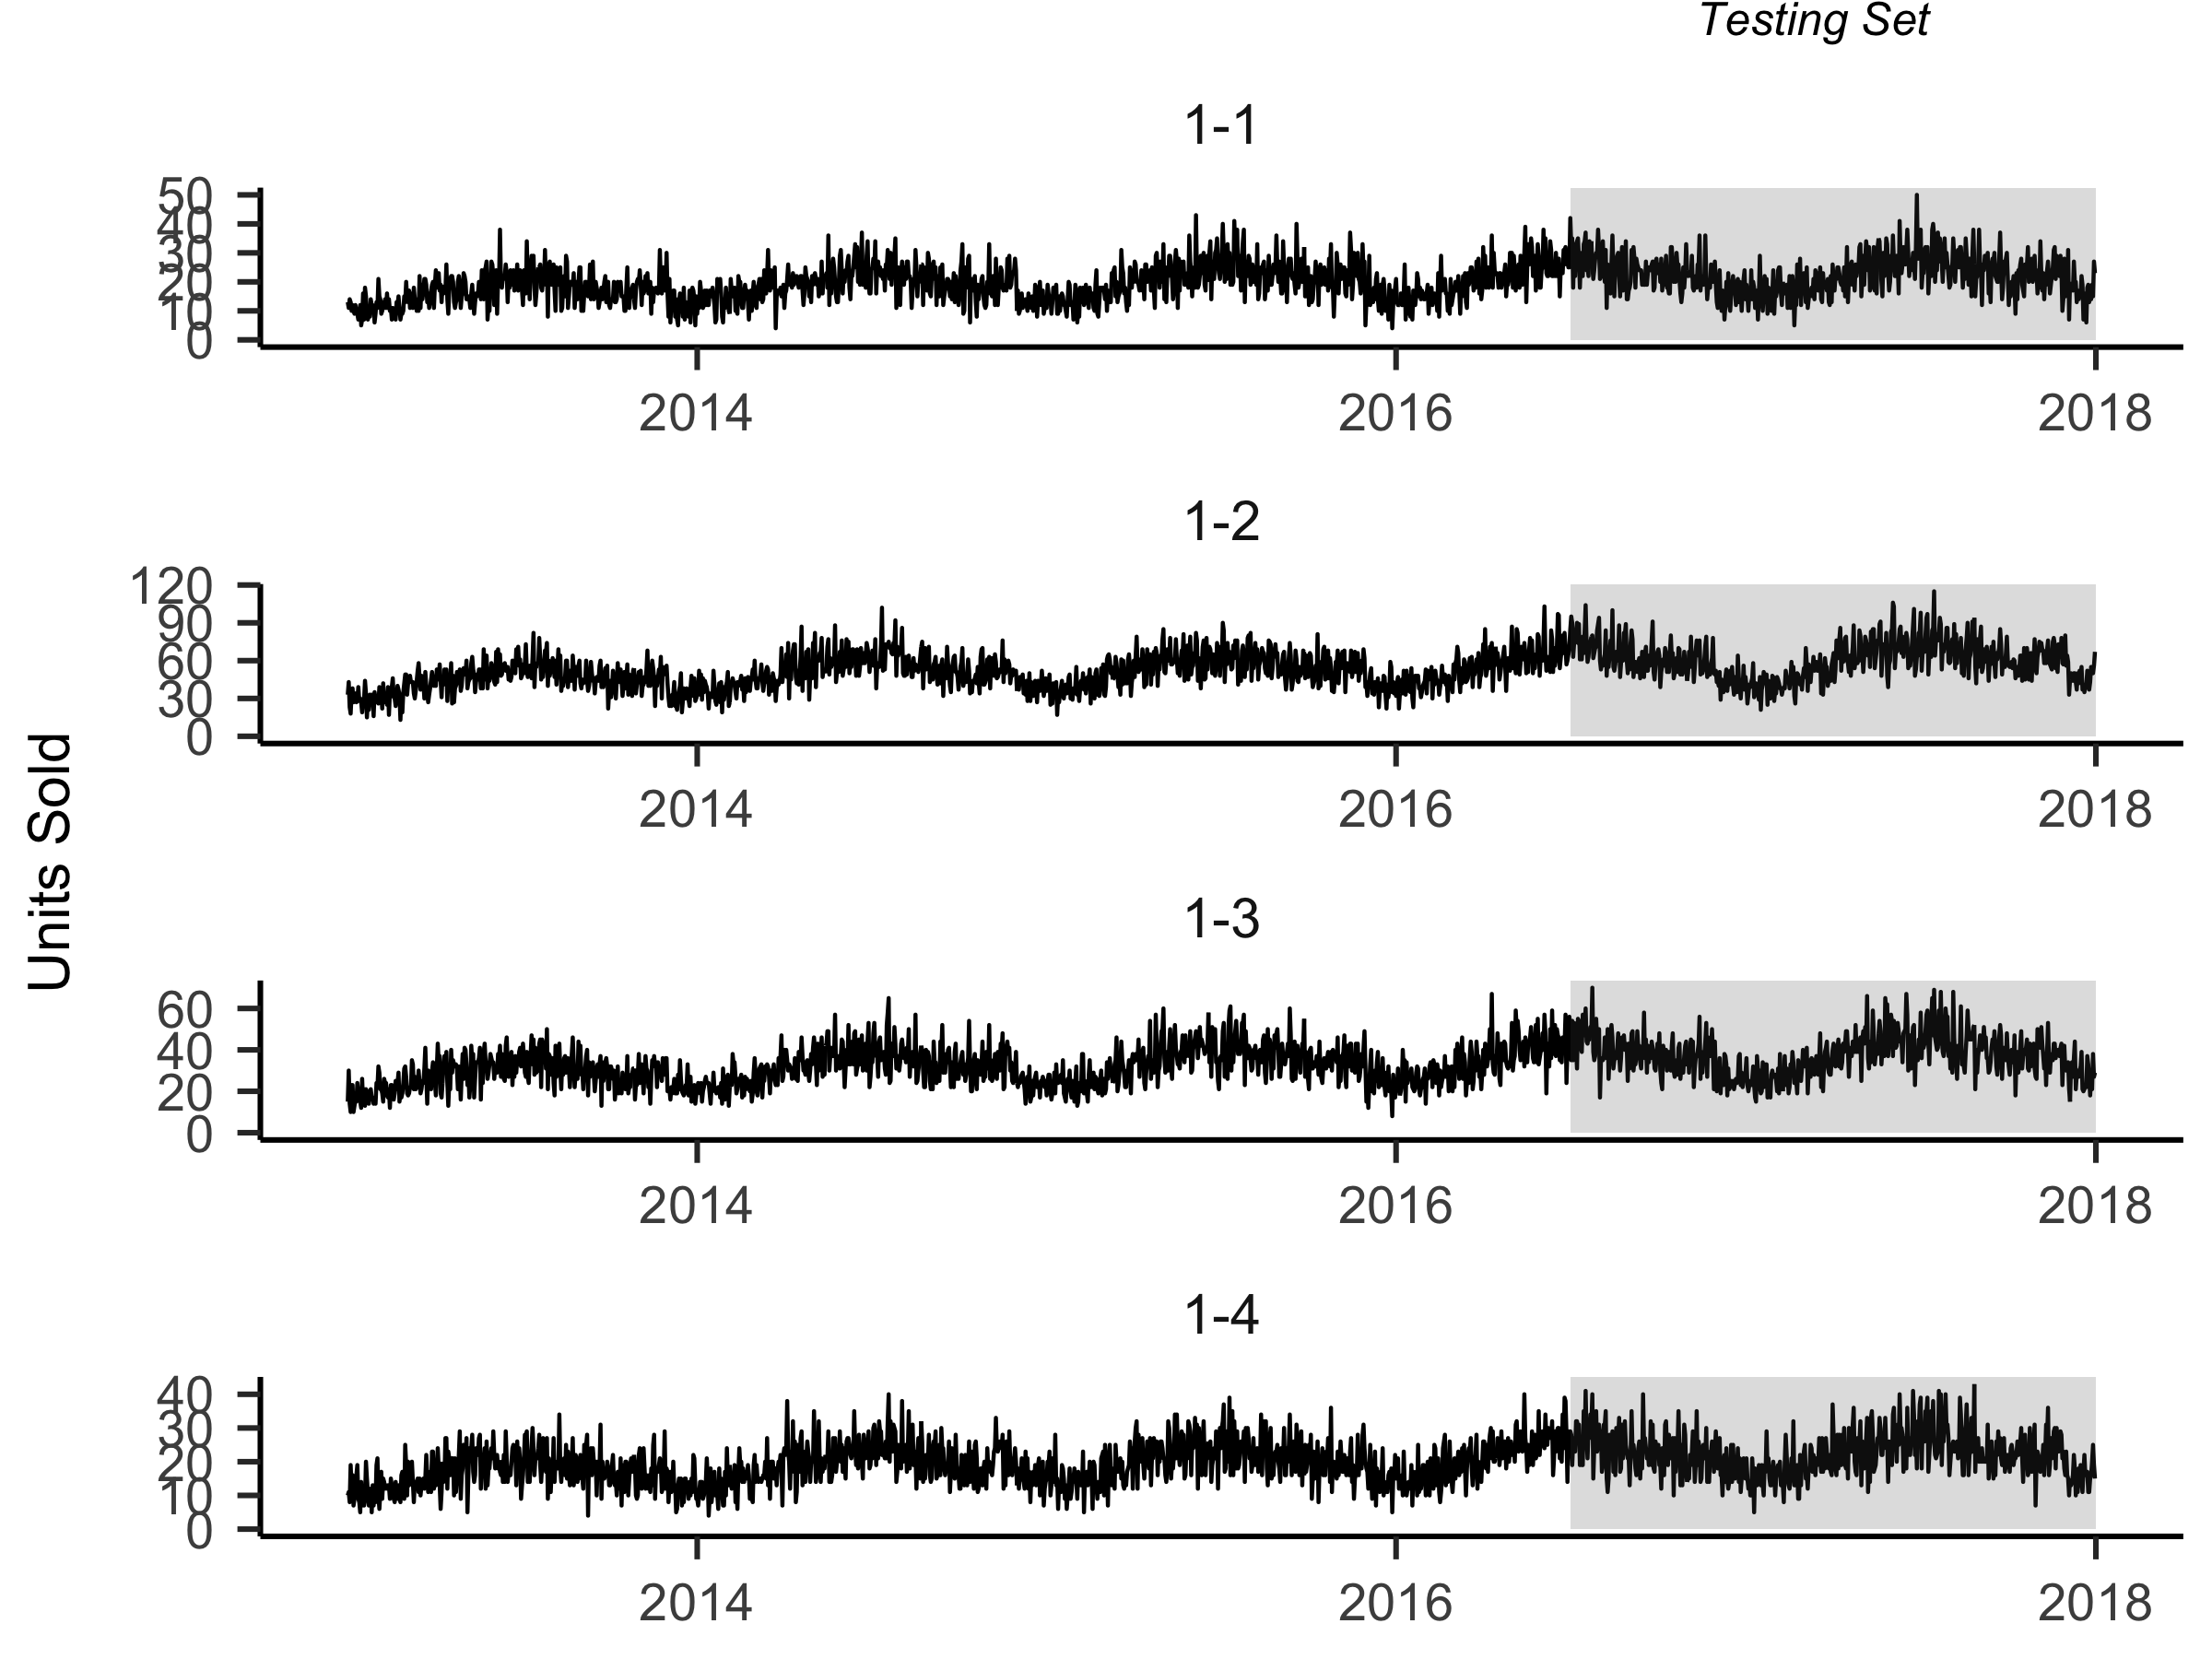
\includegraphics[width=\columnwidth]
        {plots/item_sales.png}}
	\caption{\label{fig:my-label} Daily Sales of the First Four Items in the First store}
\end{figure}

\section{Requirements}


The algorithms we select to generate high-quality forecasts will be strictly required to be fast, accurate, and interpretable. To be fast, the models must have minimal hyperparameters to tune or perform well with specified default parameters. Grid searching model parameters over many series are not feasible for this task. If these algorithms are fast, they can be ran on a wide variety of time series. That gives analysis and stakeholders a good idea of what level of performance to expect. Due to the high costs associated with forecasting errors, these models must be interpretable in the event a stakeholder has concerns with the output of a model. 

\section{Models}


We selected models that perform well in practice and fit our project requirements. We choose to test two categories of models. First, classical models are successful in practice with years of good results. They are derived with statistical methods and have strong theoretical justifications. Second, are newer machine learning-based models. We are going to test different models and evaluate them strictly on their performance on this testing data. 

\begin{table*}[t] \centering 
  \caption{Forecasting Model Performance} 
  \label{} 
\begin{tabular}{@{\extracolsep{5pt}} lrrr} 
\\[-1.8ex]\hline 
\hline \\[-1.8ex] 
Model & Daily Forecast & Aggregated Weekly & Aggregated Monthly \\ 
\hline \\[-1.8ex] 
FB Prophet & $12.890$ & $7.330$ & $4.240$ \\ 
ARDL & $16.830$ & $8.940$ & $4.480$ \\ 
Neural Prophet & $18.440$ & $10.460$ & $7.610$ \\ 
Exponential Smoothing & $19.310$ & $14.880$ & $13.540$ \\ 
Autoregression & $23.930$ & $17.510$ & $16.250$ \\ 
XGBoost & $30.350$ & $28.850$ & $28.430$ \\ 
\hline \\[-1.8ex] 

\footnotesize{Note: Measured in SMAPE see Equation 1}\\
\end{tabular} 
\end{table*} 

\begin{enumerate}
\item Seasonal Exponential Smoothing
\item Vector Autoregression
\item Autoregressive Distributed Lag
\item XGBoost 
\item Prophet
\item Neural Prophet
\end{enumerate}


The Seasonal Exponential Smoothing model, sometimes known as the Holt-Winters method, decomposes the time-series into three components: Linear Seasonality, Linear Trend, and Gaussian noise \cite{hyndman2018forecasting}. This is a simple, interpretable model, that is fast to implement and has proven quite reliable.

\subsection{Seasonal Vector Auto Regression}

Seasonal Vector Auto Regression is an autoregressive model. This takes the first 5 lag positions and uses them as regressors, then using time-series decomposition, it models the seasonality\cite{hamilton1994}. This model is commonly used to forecast economic variables and has been known to be quite robust.

\subsection{Auto Regressive Distributed Lag}

ARDL models add to the above autoregressive model by fitting seasonality with a vector of indicator variables and trend. In this case, we are adding an explanatory variable of time and fitting the model to the lagged value of time. Although there are many forecasting models to choose from, there is not much research on when a given forecasting model outperforms another. Due to the data having strong weekly swings, we implement several models with autoregressive terms.


\subsection{XGBoost}

XGBoost is an implementation of a tree boosting system. This uses decision tree regression, and fits an ensemble of models to the data, then the residuals, then fits the residuals residuals. This ensemble of tree boosting is quite robust and performs well in a variety of different regression and classification tasks\cite{chen2015xgboost}.

\subsection{Facebook's Prophet}

Facebook released a forecasting library designed specifically to meet the challenges of generating many high-quality forecasts. The model known as Prophet is a General Additive Model \cite{taylor2018forecasting}. Consisting of three functions: trend, which fits a periodic logistic population growth model (we did not limit the growth), seasonality, which is a Fourier series fit to the remaining seasonal component, and a holiday parameter which is a vector of user-specified holiday periods, the holiday periods saw a drop in sales, however not enough to justify us specifying dates. This model has been used as the industry standard in forecasting at scale\cite{triebe2021neuralprophet}.

\subsection{NeuralProphet}

NeuralProphet, is a forecasting library that expands on Facebook's prophet. It does so by including an autoregressive term in the general additive model and uses neural networks to generate the model parameters \cite{triebe2021neuralprophet}. This is quite recently released so there is not a history of it being used in production.

\begin{table*}[ht] 
\centering 
\caption{Descriptive Statistics of Forecasting Error} 
  \label{} 
\begin{tabular}{@{\extracolsep{5pt}} lrrrr} 
\\[-1.8ex]\hline 
\hline \\[-1.8ex] 
Model & Median & Standard Deviation & 95th Percentile & 5th Percentile \\ 
\hline \\[-1.8ex] 
AR Distributed Lag & $$-$2.861$ & $10.505$ & $12.472$ & $$-$21.776$ \\ 
Exponential Smoothing & $0.704$ & $14.098$ & $26.306$ & $$-$20.514$ \\ 
Neural Prophet & $6.863$ & $10.874$ & $27.095$ & $$-$8.262$ \\ 
Prophet & $0.731$ & $8.660$ & $14.355$ & $$-$13.956$ \\ 
Vector Autoreg & $$-$7.500$ & $14.374$ & $12.627$ & $$-$34.667$ \\ 
XGBoost Forecast & $$-$11.973$ & $12.889$ & $3.153$ & $$-$38.347$ \\ 
\hline \\[-1.8ex] 
\footnotesize{}\\
\end{tabular} 
\end{table*} 

\section{Performance}
Stakeholders are often far more concerned with weekly or monthly forecasts. The selected forecasting models varied in performance quite dramatically see Table 1 for the SMAPE of each model. Although there are 500 series, this is a retail sales demand that exhibits similar patterns. Therefore, we cannot speak to the validity of each model only about the performance on this testing set. Of the selected models, Facebook's prophet outperformed the rest at each level of aggregation. This is not surprising as it is precisely designed for the task of forecasting at scale \cite{taylor2018forecasting}. As the level of aggregation increases, we observe lower errors. 

An advantage of forecasting at this scale is that it shows the level of model performance to expect. See histograms of testing set errors in Figure 2. Notice, XGBoost was consistently forecasting lower than the actual value where  NeuralProphet was over forecasting. There may be applications where over or under forecasting may be preferred; however, we are looking for the most accurate models. Also, those adjustments should be made heuristically. 


\begin{figure}[!htb]
	\center{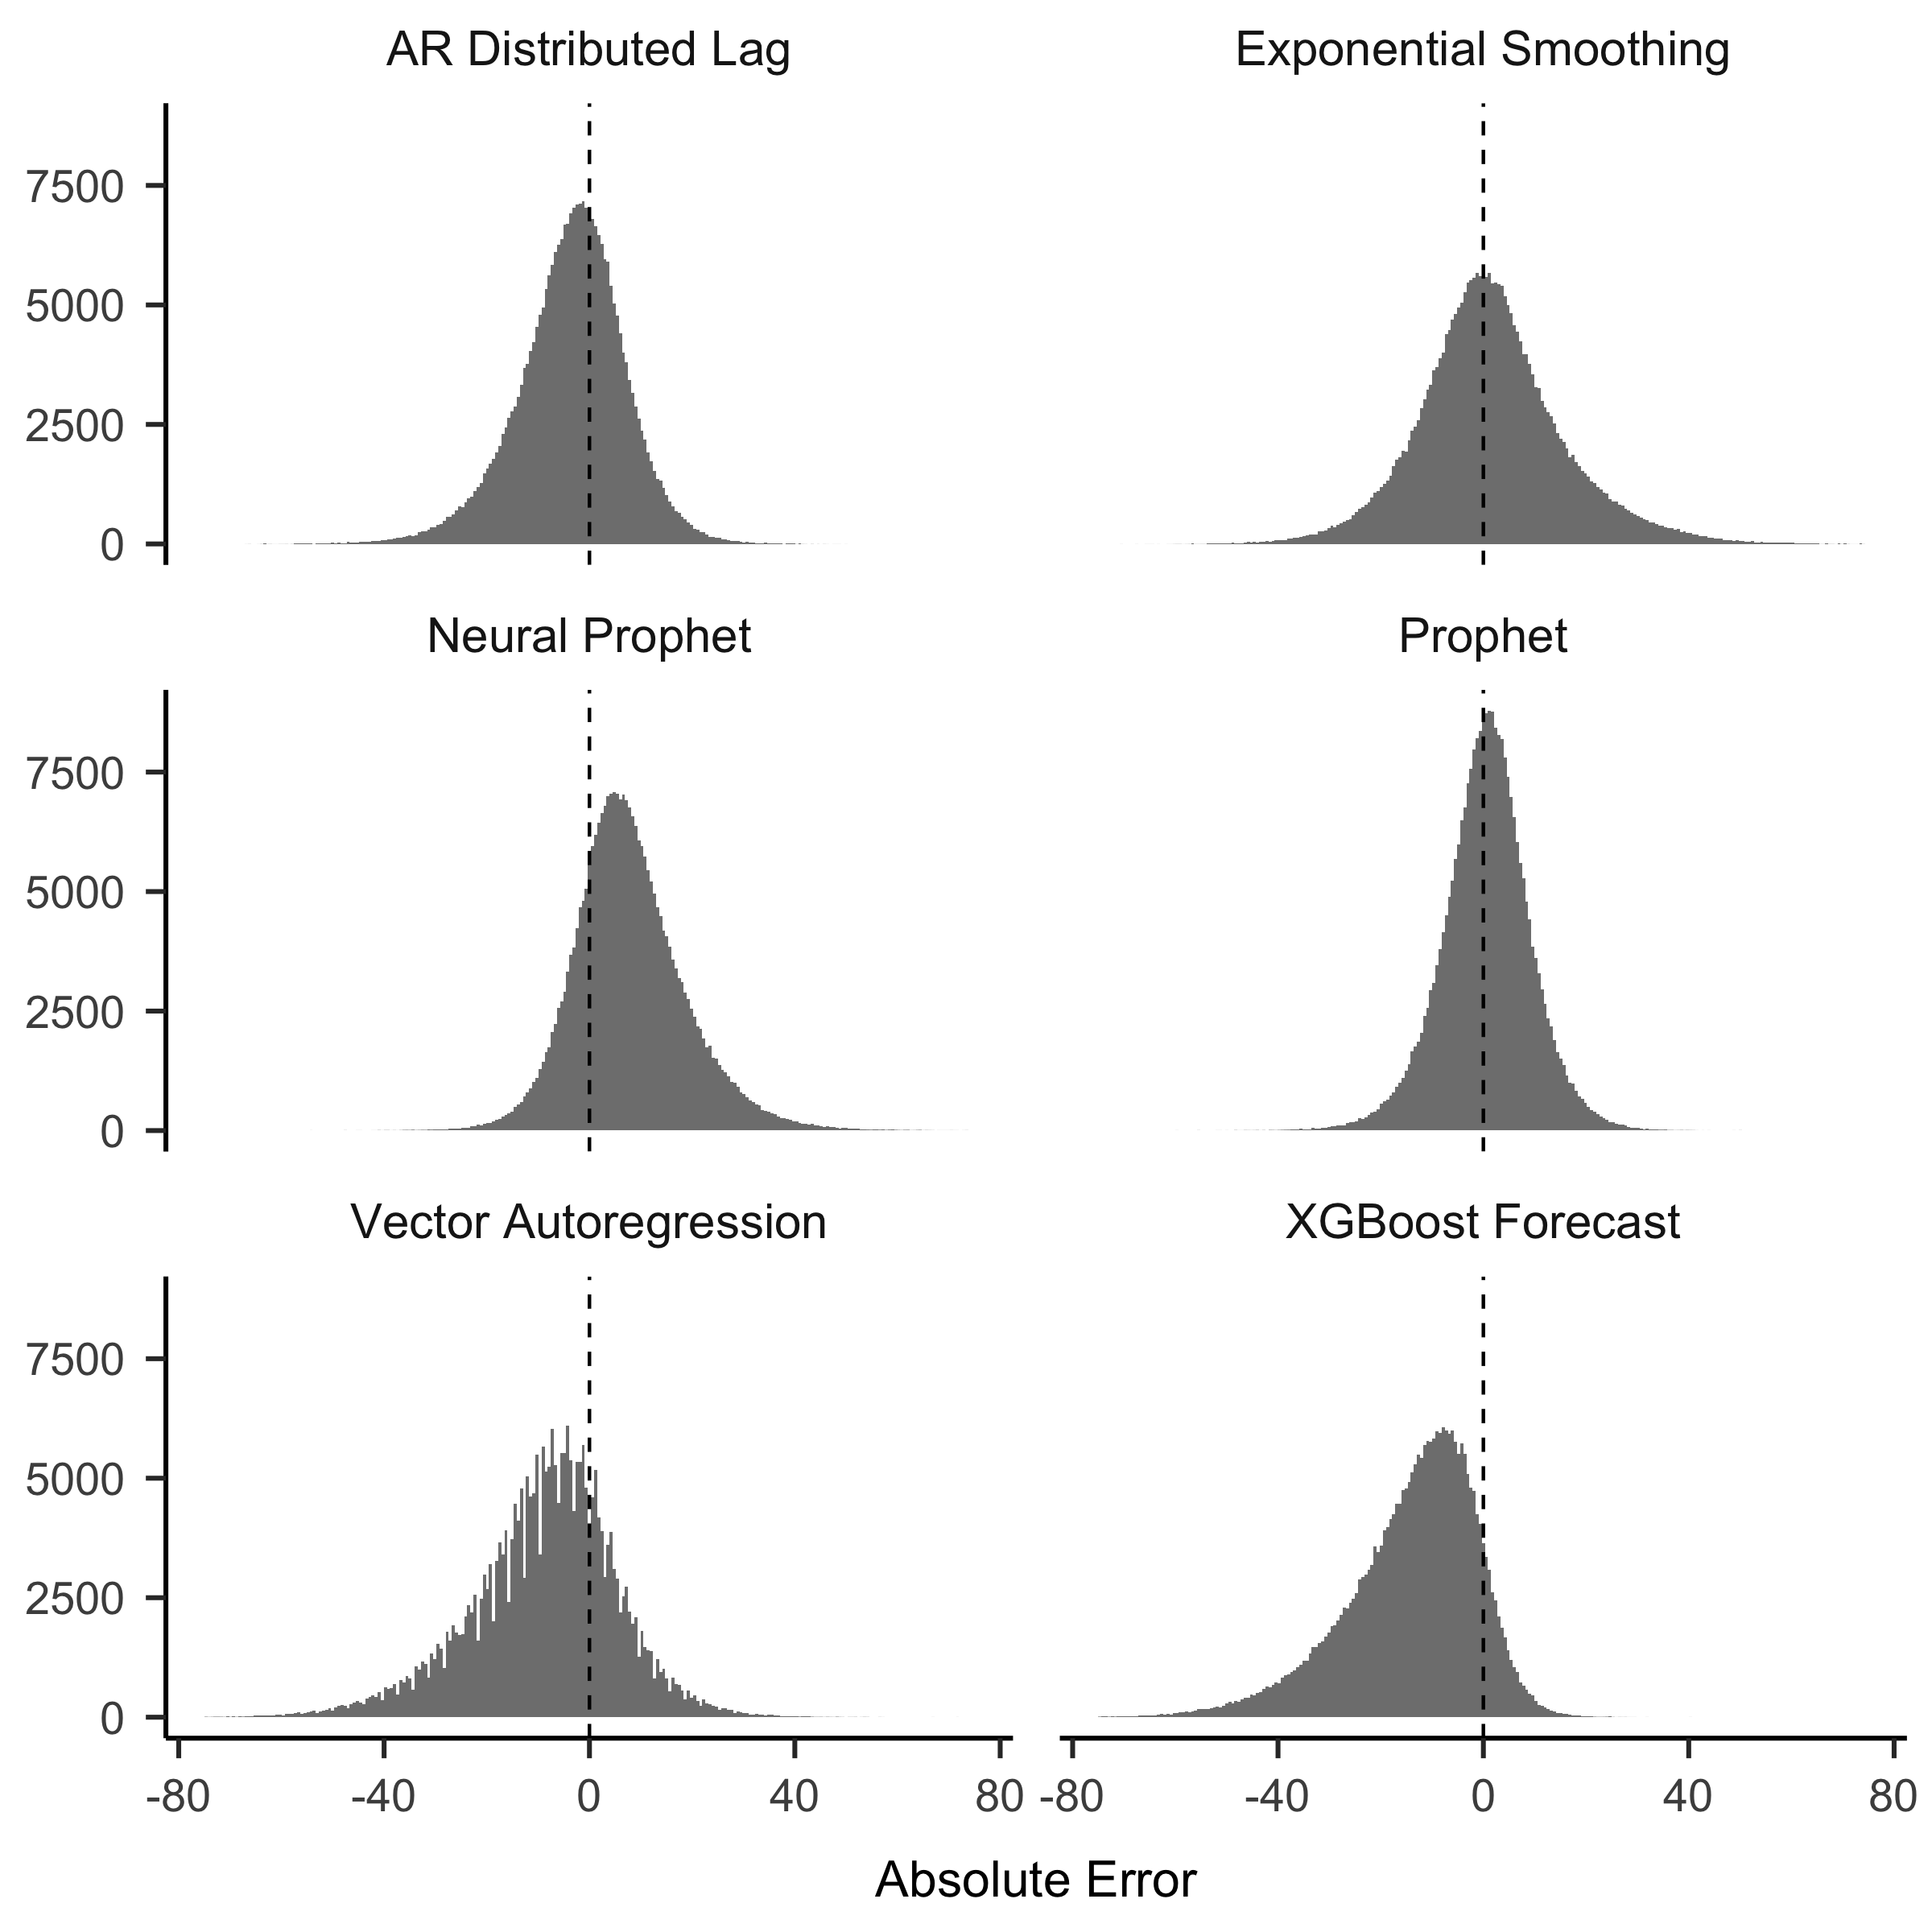
\includegraphics[width=\columnwidth]
        {plots/errors.png}}
	\caption{\label{fig:my-label} Distribution of forecasting errors}
\end{figure}

Table 2 contains descriptive statistics of each model's performance. Note the median error of Prophet was much lower than all the other models except for Exponential smoothing. Another consideration is the standard deviation of forecasting errors. This is an important consideration depending on the application. Low standard deviation in forecasting error is highly desirable because the lower the standard deviation, the more reliable. Of the models tested, Prophet had the best performance in SMAPE, had the median near zero, and the lowest standard deviation of error. 



\section{Kaggle Challenge}

In this section, we discuss the results of our attempts at this challenge. The challenge is simple, generate the best daily forecasts measured by SMAPE. Since we are not limited in entries, we attempt a variety of methods. The challenge has passed, so we have access to the leaderboards. The top score is a SMAPE of 12.07 \cite{kaggle}. Therefore, we will compare performance to that.


\begin{enumerate}
\item Weight an Average Based on Features
\item Just Use Prophet
\item Ensamble of the Top Three Models
\end{enumerate}

\subsection{Weighted Average}

Improving current models can prove very valuable. Therefore, we will attempt some machine learning methods to combine the models. The goal is to use machine learning to predict when a given forecast will be more accurate than all the others. Therefore, we will employ a feature detection algorithm combined with testing set performance to classify which model is the most accurate given the features. There are many different shapes and patterns a time-series plot can take. Seasonality, flat points, noise, and many others are quantified in the Tsfeatures package \cite{montero2020fforma}. We ran this algorithm on each series collecting 30 quantified features. The central question of this study is to determine if we can identify which forecasting model will perform the best given these features.

Using different models, we tried KNN, logistic regression, XGBoost, and an artificial neural network. The algorithms were able to select the best with an accuracy of 0.285. We used the output probabilities to take a weighted average of the models and submitted it to the challenge.

Compared to the top score on Kaggle, this method wildly underperformed scoring a SMAPE of 20.74. This is worse than nearly all the models performing on the testing data. Since we do not have access to the testing data, we cannot be sure what went wrong. We suspect is that combining all the forecasts in a weighted average smoothed out all the noise and was not able to capture daily swings.


\subsection{Just Use Prophet}

After that, there is the most simple submission. That is to simply use the top-performing model and submit the result. The Prophet model scored a SMAPE of 14.10. However, the deviation from the testing set performance is a cause for concern. It is a full two points worse than the testing set. We speculate that it is because the challenge data starts at the point of the lowest seasonality for these products and the model missed the inflection. Regardless, this method should be considered given the simplicity and accuracy of this single model. 

\subsection{Ensemble of the Top Three Models}

Given a weak performance of the weighted average and the strong performance of the Prophet model, we investigate one more approach. This method is going to use a selected ensemble of ARDL, Prophet, and Neural Prophet. We will use the probability weights from machine learning to predict the most accurate model for each given day. Then rather than taking an average, we just select that model with the highest probability of being the best. This method received a score of 14.58. This is not as accurate as just using Prophet. Additionally, it is far more complicated. 


\section{Conclusions}

Facebook's Prophet forecasting model got, by far, the best results. It was developed specifically for the task of forecasting at a scale far beyond even this project. We did not find a good way of combining the forecasts into a more accurate model. Additional studies with more data on exogenous factors could be used to combine forecasting models in a better way. Additionally, optimizing and tuning forecasting accuracy for weekly or monthly would likely produce more accurate results. 

Additionally, consider that the data set used is unusually clean with highly pronounced seasonality. Therefore, XGboost and Neural Prophet should not be discarded based on this project. Depending on the forecasting application, it may be worthwhile to tune those model parameters.



\clearpage
\onecolumn

\bibliography{References}

\end{document}